\documentclass[aspectratio=169, 12pt]{beamer}
\usepackage{fontspec}
\setmainfont{Arial}

\usetheme{Madrid}
\usecolortheme{default}

\usepackage{graphicx}
\usepackage{amsmath}
\usepackage{listings}
\usepackage{booktabs}
\usepackage{xcolor}
\usepackage{tabularx}
\usepackage{caption}

% Set code listing style
\lstset{
    basicstyle=\ttfamily\scriptsize,
    breaklines=true,
    keywordstyle=\color{blue},
    stringstyle=\color{red},
    commentstyle=\color{green!60!black},
    showstringspaces=false,
    frame=single,
    backgroundcolor=\color{gray!10}
}

\title[ML - Chap 18]{Chương 18: Học Tăng Cường (Reinforcement Learning)}
\author[Giảng viên]{Giảng viên}
\institute[Đại học Đông Á]{Đại học Đông Á}
\date{\today}

\begin{document}

% 1
\begin{frame}
    \titlepage
\end{frame}

% 2
\begin{frame}{Mục tiêu của Chương}
    \begin{itemize}
        \item Nắm vững khái niệm cơ bản về Học Tăng Cường: \textbf{Tác nhân, Môi trường, Phần thưởng}.
        \item Hiểu nguyên lý và cách tìm kiếm chính sách (Policy Search).
        \item Phân tích và áp dụng thuật toán \textbf{Học Q (Q-Learning)} thông qua bảng.
        \item Khám phá sức mạnh của \textbf{Deep Q-Learning (DQN)} và các kỹ thuật giúp nó hội tụ.
        \item Nắm bắt cơ sở lý thuyết toán học của \textbf{Markov Decision Processes (MDP)}.
        \item Triển khai mạng nơ-ron học \textbf{Độ dốc chính sách (Policy Gradients)}.
    \end{itemize}
\end{frame}

% 3
\begin{frame}{Mục lục}
    \tableofcontents
\end{frame}

%==================================================================
\section{1. Học để tối ưu hóa phần thưởng \& Tìm kiếm chính sách}
%==================================================================

% 4
\begin{frame}{1.1 Bối cảnh của Học Tăng Cường}
    \begin{itemize}
        \item Trong Học Máy, chúng ta đã quen với \textbf{Học có giám sát} (có nhãn sẵn) và \textbf{Học không giám sát} (tìm quy luật).
        \item \textbf{Học Tăng Cường (Reinforcement Learning - RL)} là một mô hình hoàn toàn khác.
        \item Nó xoay quanh một hệ thống đang tự động học hỏi bằng cách \textit{tương tác} với môi trường xung quanh.
        \item Mục tiêu duy nhất: Tối đa hóa tổng \textbf{Phần thưởng (Reward)} nhận được theo thời gian.
    \end{itemize}
\end{frame}

% 5
\begin{frame}{1.2 Mô hình Tác nhân và Môi trường}
    \begin{columns}
        \begin{column}{0.4\textwidth}
            \begin{itemize}
                \item \textbf{Tác nhân (Agent):} Chủ thể quan sát và đưa ra quyết định (VD: Robot, phần mềm chơi cờ).
                \item \textbf{Môi trường (Environment):} Thế giới vật lý hoặc giả lập mà Tác nhân thao tác.
                \item Môi trường cung cấp \textbf{Trạng thái} và \textbf{Phần thưởng}. Tác nhân tác động lại bằng \textbf{Hành động}.
            \end{itemize}
        \end{column}
        \begin{column}{0.6\textwidth}
            \centering
            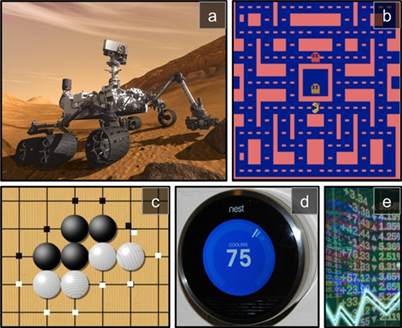
\includegraphics[width=\textwidth,height=0.65\textheight,keepaspectratio]{../machineLearningWeb/Figures/CH18/Hình_18-1.png}
            \vspace{0.2cm}
            \textit{Hình 18-1: Chu trình Học Tăng Cường cơ bản}
        \end{column}
    \end{columns}
\end{frame}

% 6
\begin{frame}{1.3 Ví dụ thực tế về RL}
    \begin{itemize}
        \item \textbf{Điều khiển Robot:} Robot học cách đi bộ. Nếu đi được, +1 điểm. Nếu ngã, -10 điểm. Qua hàng triệu lần ngã, nó tự biết cách thăng bằng.
        \item \textbf{Chơi Game:} AlphaGo của DeepMind đánh bại nhà vô địch thế giới cờ vây Lee Sedol. Phần thưởng chỉ được trao ở cuối ván (Thắng = +1, Thua = -1).
        \item \textbf{Quản lý danh mục đầu tư:} Tác nhân mua/bán cổ phiếu dựa trên trạng thái thị trường. Phần thưởng là lợi nhuận thu về.
    \end{itemize}
\end{frame}

% 7
\begin{frame}{1.4 Chính sách (Policy)}
    \begin{itemize}
        \item \textbf{Chính sách (ký hiệu là $\pi$):} Là thuật toán hoặc hàm số mà Agent dùng để ra quyết định.
        \item Phân loại chính sách:
        \begin{itemize}
            \item \textbf{Chính sách xác định (Deterministic Policy):} Ở trạng thái S, luôn chọn hành động A (VD: $A = \pi(S)$).
            \item \textbf{Chính sách ngẫu nhiên (Stochastic Policy):} Ở trạng thái S, có 80\% chọn A, 20\% chọn B.
        \end{itemize}
        \item Nhiệm vụ cốt lõi của RL là đi tìm một chính sách tối ưu $\pi^*$.
    \end{itemize}
\end{frame}

% 8
\begin{frame}{1.5 Tìm kiếm chính sách (Policy Search)}
    \begin{columns}
        \begin{column}{0.45\textwidth}
            \begin{itemize}
                \item Không gian của tất cả các chính sách có thể có là vô cùng tận. Làm sao để tìm ra chính sách tốt?
                \item \textbf{Cách tiếp cận:}
                \item 1. \textit{Tìm kiếm ngẫu nhiên:} Đặt tham số mạng nơ-ron ngẫu nhiên, cho chạy thử. Rất kém hiệu quả.
                \item 2. \textit{Thuật toán di truyền:} Lai ghép các chính sách tốt.
                \item 3. \textit{Gradient Ascent:} Dùng đạo hàm để leo lên đỉnh núi phần thưởng.
            \end{itemize}
        \end{column}
        \begin{column}{0.55\textwidth}
            \centering
            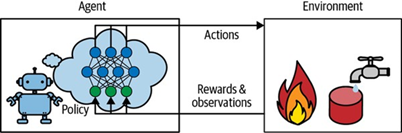
\includegraphics[width=\textwidth,height=0.65\textheight,keepaspectratio]{../machineLearningWeb/Figures/CH18/Hình_18-2.png}
            \vspace{0.2cm}
            \textit{Hình 18-2: Không gian chính sách và quá trình tìm đỉnh}
        \end{column}
    \end{columns}
\end{frame}

% 9
\begin{frame}{1.6 Môi trường OpenAI Gym (Gymnasium)}
    \begin{itemize}
        \item Để huấn luyện AI, ta cần một môi trường giả lập chuẩn hóa.
        \item \textbf{OpenAI Gym} ra đời để cung cấp một API thống nhất cho hàng loạt các môi trường khác nhau.
        \item Các bước tương tác cơ bản với Gym:
        \begin{itemize}
            \item \texttt{env.reset()}: Khởi động lại môi trường.
            \item \texttt{env.step(action)}: Yêu cầu môi trường thực thi hành động. Trả về: (state, reward, done, info).
        \end{itemize}
    \end{itemize}
\end{frame}

% 10
\begin{frame}[fragile]{1.7 Cấu trúc Code cơ bản với OpenAI Gym}
\begin{lstlisting}[language=Python]
import gym

env = gym.make("CartPole-v1")
obs = env.reset()

for step in range(1000):
    env.render()  # Hien thi hinh anh
    action = env.action_space.sample()  # Chon hanh dong ngau nhien
    obs, reward, done, info = env.step(action)
    
    if done:
        print(f"Game over sau {step} buoc!")
        break
env.close()
\end{lstlisting}
    \begin{itemize}
        \item \textit{Code minh họa một Agent ngốc nghếch chọn hành động hoàn toàn ngẫu nhiên.}
    \end{itemize}
\end{frame}

% 11
\begin{frame}{1.8 Bài toán CartPole}
    \begin{columns}
        \begin{column}{0.45\textwidth}
            \begin{itemize}
                \item \textbf{Nhiệm vụ:} Giữ gậy đứng thẳng trên chiếc xe.
                \item \textbf{Không gian hành động:}
                    \begin{itemize}
                        \item 0: Đẩy sang trái
                        \item 1: Đẩy sang phải
                    \end{itemize}
                \item \textbf{Không gian quan sát (Observation):} [Vị trí xe, Vận tốc xe, Góc nghiêng gậy, Vận tốc góc].
                \item \textbf{Done (Kết thúc):} Khi gậy nghiêng quá $15^\circ$ hoặc xe chạy ra khỏi màn hình.
            \end{itemize}
        \end{column}
        \begin{column}{0.55\textwidth}
            \centering
            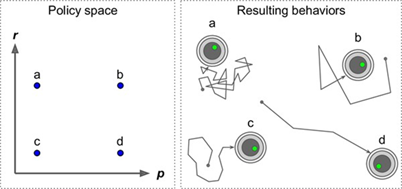
\includegraphics[width=\textwidth,height=0.65\textheight,keepaspectratio]{../machineLearningWeb/Figures/CH18/Hình_18-3.png}
            \vspace{0.2cm}
            \textit{Hình 18-3: Giao diện giả lập CartPole}
        \end{column}
    \end{columns}
\end{frame}

% 12
\begin{frame}{1.9 Các Chính sách bằng Mạng Nơ-ron}
    \begin{itemize}
        \item Thay vì dùng If-Else, ta dùng một \textbf{Mạng Nơ-ron MLP} (Multi-Layer Perceptron) để làm Chính sách.
        \item Đầu vào: Một mảng các quan sát (Ví dụ: 4 giá trị của CartPole).
        \item Lớp ẩn: Xử lý thông tin phi tuyến.
        \item Đầu ra: Xác suất chọn các hành động (Dùng hàm Softmax cho đa lớp, hoặc Sigmoid cho nhị phân).
        \item Trọng số của mạng sẽ được cập nhật liên tục qua quá trình huấn luyện.
    \end{itemize}
\end{frame}

% 13
\begin{frame}{1.10 Bài toán Phân bổ tín nhiệm (Credit Assignment)}
    \begin{itemize}
        \item Khi đánh cờ, bạn thực hiện 100 nước đi. Đến nước thứ 101, bạn chiến thắng và nhận thưởng +100.
        \item Cả 100 nước đi đó đều là nước tốt? Chưa chắc, có thể nước 50 rất tệ nhưng nước 99 cực kỳ xuất sắc.
        \item \textbf{Làm thế nào để hệ thống biết chính xác hành động nào trong quá khứ xứng đáng được biểu dương (phân bổ tín nhiệm)?}
        \item Giải pháp phổ biến: Sử dụng hệ số chiết khấu và thuật toán \textit{Truy ngược phần thưởng (Reward Backpropagation)}.
    \end{itemize}
\end{frame}


%==================================================================
\section{2. Markov Decision Processes (MDP)}
%==================================================================

% 14
\begin{frame}{2.1 Nền tảng Toán học: Quá trình Markov}
    \begin{itemize}
        \item \textbf{Quá trình Markov (Markov Chain):} Một hệ thống chuyển đổi giữa các trạng thái theo xác suất cố định, không có bộ nhớ (Memoryless).
        \item "Tương lai chỉ phụ thuộc vào trạng thái hiện tại, không liên quan đến quá khứ".
        \item Trạng thái thời tiết: Từ Nắng $\rightarrow$ có 70\% sang Mưa, 30\% tiếp tục Nắng.
    \end{itemize}
\end{frame}

% 15
\begin{frame}{2.2 Quá trình Quyết định Markov (MDP)}
    \begin{columns}
        \begin{column}{0.5\textwidth}
            \begin{itemize}
                \item MDP là bản nâng cấp của Markov Chain, bổ sung thêm 2 thành phần cốt lõi:
                \begin{itemize}
                    \item \textbf{Hành động (Action):} Ta có quyền can thiệp vào quá trình chuyển trạng thái.
                    \item \textbf{Phần thưởng (Reward):} Nhận được sau khi chuyển trạng thái.
                \end{itemize}
                \item Đây là cách biểu diễn toán học chuẩn xác nhất cho mọi bài toán RL.
            \end{itemize}
        \end{column}
        \begin{column}{0.5\textwidth}
            \centering
            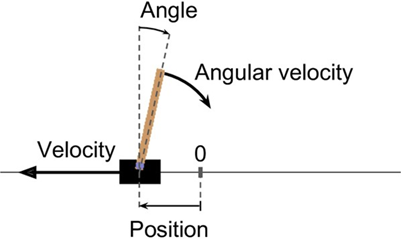
\includegraphics[width=\textwidth,height=0.65\textheight,keepaspectratio]{../machineLearningWeb/Figures/CH18/Hình_18-4.png}
            \vspace{0.2cm}
            \textit{Hình 18-4: Sơ đồ minh họa MDP với Trạng thái, Hành động và Xác suất}
        \end{column}
    \end{columns}
\end{frame}

% 16
\begin{frame}{2.3 Hệ số chiết khấu (Discount Factor - $\gamma$)}
    \begin{itemize}
        \item Agent không chỉ tìm kiếm phần thưởng lập tức, mà phải tối ưu phần thưởng dài hạn.
        \item Tuy nhiên, 10 điểm ngay bây giờ luôn chắc chắn hơn 10 điểm vào tuần sau.
        \item Ta định nghĩa \textbf{Lợi nhuận (Return $G_t$)} tại bước $t$:
        $$ G_t = R_{t+1} + \gamma R_{t+2} + \gamma^2 R_{t+3} + \dots $$
        \item $\gamma$ (gamma) thường lấy giá trị từ 0.9 đến 0.99. Nếu $\gamma=0$, Agent rất thiển cận (chỉ nhìn trước mắt). Nếu $\gamma \rightarrow 1$, Agent nhìn xa trông rộng.
    \end{itemize}
\end{frame}

% 17
\begin{frame}{2.4 Đánh giá Trạng thái và Hành động}
    \begin{itemize}
        \item Làm sao để biết một trạng thái $S$ là tốt hay xấu?
        \item \textbf{Hàm giá trị trạng thái (State-Value Function - $V^\pi(s)$):} Tính tổng lợi nhuận dự kiến nhận được nếu bắt đầu từ $s$ và tuân theo chính sách $\pi$.
        \item \textbf{Hàm giá trị hành động (Action-Value Function - $Q^\pi(s,a)$):} Đứng ở $s$, thực hiện hành động $a$, sau đó tuân theo chính sách $\pi$, thì thu được bao nhiêu?
    \end{itemize}
\end{frame}

% 18
\begin{frame}{2.5 Phương trình Bellman (Bellman Equation)}
    \begin{itemize}
        \item Richard Bellman đã chứng minh được mối liên hệ đệ quy của các hàm Giá trị:
        \item Để tính $V(s)$ tại trạng thái hiện tại, ta chỉ cần phần thưởng ngay lập tức và $V(s')$ của trạng thái tiếp theo:
        $$ V^*(s) = \max_a \left[ R(s,a) + \gamma \sum_{s'} P(s'|s,a) V^*(s') \right] $$
        \item Công thức này cho phép ta giải bài toán bằng \textbf{Quy hoạch động (Dynamic Programming)} hoặc vòng lặp.
    \end{itemize}
\end{frame}


%==================================================================
\section{3. Học Q (Q-Learning) Cổ điển}
%==================================================================

% 19
\begin{frame}{3.1 Nguyên lý Học Q (Q-Learning)}
    \begin{itemize}
        \item Q-Learning (đề xuất năm 1989 bởi Watkins) không cần biết trước môi trường (Model-free).
        \item Thuật toán lưu trữ tất cả các giá trị $Q(s, a)$ vào một cái Bảng khổng lồ (Q-Table).
        \item Ban đầu Q-Table chứa toàn số 0. Agent bắt đầu đi lung tung.
        \item Mỗi lần bước đi, nó cập nhật Q-Table dựa trên \textbf{Chênh lệch Thời gian (Temporal Difference - TD)}.
    \end{itemize}
\end{frame}

% 20
\begin{frame}{3.2 Công thức Cập nhật Q-Learning}
    \begin{itemize}
        \item Tại mỗi bước, khi đi từ $S \rightarrow S'$ với hành động $A$, nhận phần thưởng $R$:
        $$ Q(s, a) \leftarrow Q(s, a) + \alpha \left[ R + \gamma \max_{a'} Q(s', a') - Q(s, a) \right] $$
        \item Trong đó:
            \begin{itemize}
                \item $\alpha$ (Alpha): Tốc độ học (Learning Rate).
                \item $R + \gamma \max Q(s', a')$: \textbf{Mục tiêu TD (TD Target)} (Giá trị thực tế vừa nhận).
                \item $\left[ \dots \right]$: \textbf{Sai số TD (TD Error)} (Dự đoán sai bao nhiêu).
            \end{itemize}
        \item Agent học bằng cách liên tục thu hẹp sai số TD.
    \end{itemize}
\end{frame}

% 21
\begin{frame}{3.3 Vấn đề: Khám phá hay Khai thác (Exploration vs Exploitation)}
    \begin{itemize}
        \item Nếu Agent luôn chọn hành động có Q-value lớn nhất (Khai thác), nó sẽ mắc kẹt.
        \item Ví dụ: Nó tìm thấy một con đường đi an toàn được +5 điểm. Nó cứ đi mãi đường đó. Trong khi đường khác tuy mạo hiểm nhưng được +100 điểm, nó lại không bao giờ khám phá ra.
        \item Do đó, ta phải \textbf{ép} hệ thống có một tỷ lệ Khám phá ngẫu nhiên (Exploration).
    \end{itemize}
\end{frame}

% 22
\begin{frame}{3.4 Chính sách Epsilon-Greedy}
    \begin{columns}
        \begin{column}{0.45\textwidth}
            \begin{itemize}
                \item \textbf{Epsilon-Greedy:}
                \item Đặt một biến $\epsilon = 1.0$ (100\% ngẫu nhiên).
                \item Sinh ra một số ngẫu nhiên từ $0-1$.
                \item Nếu số đó $< \epsilon$: Chọn hành động ngẫu nhiên.
                \item Nếu $> \epsilon$: Chọn hành động tốt nhất trong Q-Table (Khai thác).
                \item $\epsilon$ sẽ giảm dần theo thời gian (ví dụ giảm xuống $0.05$).
            \end{itemize}
        \end{column}
        \begin{column}{0.55\textwidth}
            \centering
            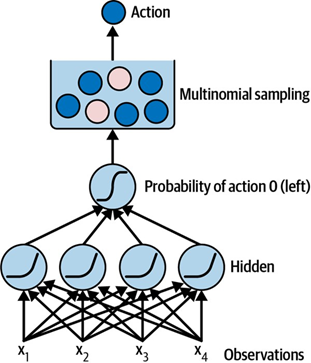
\includegraphics[width=\textwidth,height=0.65\textheight,keepaspectratio]{../machineLearningWeb/Figures/CH18/Hình_18-5.png}
            \vspace{0.2cm}
            \textit{Hình 18-5: Chiến lược giảm dần tỷ lệ Epsilon theo thời gian}
        \end{column}
    \end{columns}
\end{frame}


%==================================================================
\section{4. Học Q Sâu (Deep Q-Learning)}
%==================================================================

% 23
\begin{frame}{4.1 Khi Không Gian Trạng Thái Quá Lớn}
    \begin{itemize}
        \item Q-Table cực kỳ tốn RAM. Nếu trò chơi Pacman lấy hình ảnh làm trạng thái (VD: ảnh $210 \times 160$ pixel với 256 màu), số lượng trạng thái là $256^{210 \times 160}$.
        \item Máy tính không thể tạo mảng 2 chiều có kích thước này.
        \item Giải pháp mang tính đột phá của DeepMind (2013): \textbf{Học Q Xấp xỉ (Approximate Q-Learning)}. Dùng Mạng Nơ-ron (DQN) để đoán Q-value.
    \end{itemize}
\end{frame}

% 24
\begin{frame}{4.2 Kiến trúc Deep Q-Network (DQN)}
    \begin{columns}
        \begin{column}{0.4\textwidth}
            \begin{itemize}
                \item Mạng DQN nhận \textbf{Đầu vào} là Hình ảnh màn hình Game.
                \item Đi qua các lớp \textbf{Convolutional (CNN)} để trích xuất đặc trưng.
                \item \textbf{Đầu ra} là một lớp Dense với số nơ-ron bằng chính số Hành động (Trái, Phải, Nhảy, Bắn). Mỗi nơ-ron xuất ra một giá trị Q.
            \end{itemize}
        \end{column}
        \begin{column}{0.6\textwidth}
            \centering
            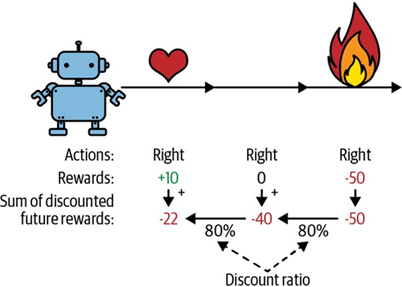
\includegraphics[width=\textwidth,height=0.7\textheight,keepaspectratio]{../machineLearningWeb/Figures/CH18/Hình_18-6.png}
            \vspace{0.2cm}
            \textit{Hình 18-6: Kiến trúc Mạng Nơ-ron Tích chập DQN chơi Atari}
        \end{column}
    \end{columns}
\end{frame}

% 25
\begin{frame}{4.3 Vấn đề Hội tụ của DQN}
    \begin{itemize}
        \item Khác với Q-Table, dùng Mạng Nơ-ron cho RL cực kỳ thiếu ổn định (Instability) và rất hay phá vỡ những gì đã học.
        \item Hai lý do chính:
        \begin{itemize}
            \item \textbf{Mẫu học có tính tương quan mạnh:} (Khung hình 1 rất giống khung hình 2). Nếu cập nhật mạng bằng dữ liệu liên tiếp, mạng sẽ "quên" cách xử lý các trường hợp xa xôi.
            \item \textbf{Mục tiêu di động:} Chúng ta đang dùng chính dự đoán của mạng để làm nhãn cho mạng học, dẫn đến vòng luẩn quẩn.
        \end{itemize}
    \end{itemize}
\end{frame}

% 26
\begin{frame}{4.4 Giải pháp 1: Trải nghiệm Phát lại (Replay Buffer)}
    \begin{itemize}
        \item Agent không học ngay sau mỗi khung hình.
        \item Nó chạy quanh trò chơi và lưu tất cả kinh nghiệm (State, Action, Reward, Next State) vào một bộ nhớ khổng lồ (Replay Memory / Buffer, sức chứa khoảng 1 triệu mẫu).
        \item Khi huấn luyện, mạng bốc ngẫu nhiên 32 mẫu từ bộ nhớ này (Mini-batch).
        \item Điều này phá vỡ tính tương quan thời gian và sử dụng hiệu quả kinh nghiệm (1 mẫu được học đi học lại).
    \end{itemize}
\end{frame}

% 27
\begin{frame}{4.5 Giải pháp 2: Mạng Mục tiêu (Target Network)}
    \begin{columns}
        \begin{column}{0.5\textwidth}
            \begin{itemize}
                \item Ta tạo ra 2 mạng Nơ-ron có kiến trúc y hệt nhau:
                \begin{itemize}
                    \item \textbf{Online Network:} Mạng chính liên tục học và cập nhật.
                    \item \textbf{Target Network:} Dùng để tính điểm mục tiêu (Q Target). Nó bị "đóng băng" (không cập nhật).
                \end{itemize}
                \item Cứ sau $10,000$ bước, ta copy trọng số từ Mạng Online sang Mạng Target một lần.
            \end{itemize}
        \end{column}
        \begin{column}{0.5\textwidth}
            \centering
            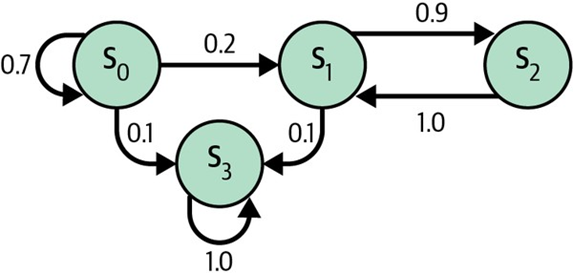
\includegraphics[width=\textwidth,height=0.6\textheight,keepaspectratio]{../machineLearningWeb/Figures/CH18/Hình_18-7.png}
            \vspace{0.2cm}
            \textit{Hình 18-7: Quá trình đồng bộ chậm từ Online sang Target}
        \end{column}
    \end{columns}
\end{frame}

% 28
\begin{frame}[fragile]{4.6 Pseudo-code cho DQN với Keras}
\begin{lstlisting}[language=Python]
# Target Network tinh toan gia tri tuong lai
next_Q_values = target_model.predict(next_states)
max_next_Q_values = np.max(next_Q_values, axis=1)

# Tính nhãn (Target) bang phuong trinh Bellman
target_Q_values = rewards + (1 - dones) * gamma * max_next_Q_values

# Mask de chi chon Q-value cua hanh dong da thuc hien
mask = tf.one_hot(actions, num_actions)

with tf.GradientTape() as tape:
    all_Q_values = model(states)
    Q_values = tf.reduce_sum(all_Q_values * mask, axis=1)
    # Tinh sai so MSE
    loss = tf.reduce_mean(keras.losses.mean_squared_error(target_Q_values, Q_values))
\end{lstlisting}
\end{frame}

% 29
\begin{frame}{4.7 Cải tiến của DQN: Double DQN}
    \begin{itemize}
        \item Mạng DQN truyền thống có xu hướng \textbf{đánh giá quá cao (Overestimate)} giá trị thật sự.
        \item Khi lấy $\max Q$ để làm mục tiêu, nó vô tình chọn những nơ-ron đang bị "ảo tưởng" (Nhiễu tích cực).
        \item \textbf{Double DQN:}
        \begin{itemize}
            \item Dùng \textbf{Mạng Online} để quyết định Đâu là hành động tốt nhất.
            \item Dùng \textbf{Mạng Target} để tính Giá trị thực sự của hành động đó.
            \item Tách bạch người đánh giá và người chọn hành động!
        \end{itemize}
    \end{itemize}
\end{frame}

% 30
\begin{frame}{4.8 Cải tiến của DQN: Dueling DQN}
    \begin{columns}
        \begin{column}{0.5\textwidth}
            \begin{itemize}
                \item Tách mạng làm 2 luồng song song sau phần tích chập CNN:
                \item Luồng 1 tính Giá trị Trạng thái $V(s)$.
                \item Luồng 2 tính Lợi thế Hành động $A(s, a)$ (Hành động này tốt hơn mức trung bình bao nhiêu).
                \item Hàm kết hợp: $Q(s, a) = V(s) + A(s, a)$.
            \end{itemize}
        \end{column}
        \begin{column}{0.5\textwidth}
            \centering
            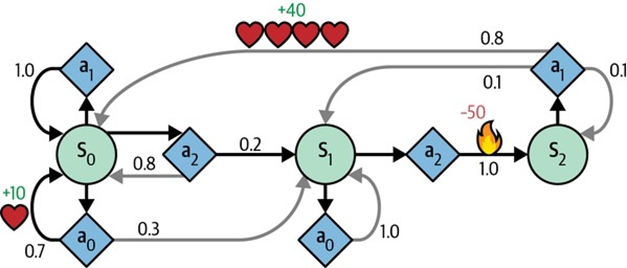
\includegraphics[width=\textwidth,height=0.65\textheight,keepaspectratio]{../machineLearningWeb/Figures/CH18/Hình_18-8.png}
            \vspace{0.2cm}
            \textit{Hình 18-8: Kiến trúc mạng DQN thông thường (trên) và Dueling DQN (dưới)}
        \end{column}
    \end{columns}
\end{frame}

% 31
\begin{frame}{4.9 Ưu tiên Trải nghiệm (Prioritized Experience Replay)}
    \begin{itemize}
        \item Khi bốc mẫu từ Replay Buffer, thay vì bốc ngẫu nhiên (Uniform), ta bốc theo \textbf{mức độ ưu tiên}.
        \item Những mẫu nào mạng dự đoán sai nhiều nhất (TD Error lớn nhất) sẽ được "chăm sóc" đặc biệt và học lại nhiều lần hơn.
        \item Giống như con người: Ta thường khắc sâu những sai lầm thảm khốc thay vì những công việc lặp đi lặp lại nhàm chán.
    \end{itemize}
\end{frame}

%==================================================================
\section{5. Độ dốc Chính sách (Policy Gradients)}
%==================================================================

% 32
\begin{frame}{5.1 Hạn chế của Học Q với Hành động Liên tục}
    \begin{itemize}
        \item Các phương pháp Q-Learning tính $Q$ cho TỪNG hành động một.
        \item Nếu hệ thống có không gian hành động liên tục (Ví dụ: Góc xoay vô-lăng từ $-90^\circ$ đến $+90^\circ$ có vô số giá trị).
        \item Làm sao có thể lấy $\max_a Q(s,a)$ với vô hạn hành động? Q-Learning sẽ sụp đổ.
        \item Ta cần đổi sang các thuật toán \textbf{Policy-Based (Dựa trên Chính sách)}.
    \end{itemize}
\end{frame}

% 33
\begin{frame}{5.2 Nguyên lý Độ dốc Chính sách (Policy Gradients - PG)}
    \begin{itemize}
        \item Không thèm tính giá trị $Q$ nữa. Mạng nơ-ron nhận đầu vào là Trạng thái, và xuất trực tiếp \textbf{Xác suất chọn hành động} (softmax) hoặc xuất trực tiếp \textbf{Giá trị liên tục} (mean, std).
        \item \textbf{Ý tưởng cốt lõi của PG:} 
        \begin{itemize}
            \item Chơi 1 ván game trọn vẹn đến cuối.
            \item Nếu kết quả chung cuộc Tốt (Phần thưởng cao), tăng xác suất của TOÀN BỘ các quyết định đã chọn trong ván đó.
            \item Nếu Tệ, giảm xác suất của chúng.
        \end{itemize}
    \end{itemize}
\end{frame}

% 34
\begin{frame}{5.3 Thuật toán REINFORCE (1992)}
    \begin{columns}
        \begin{column}{0.45\textwidth}
            \begin{itemize}
                \item Thuật toán kinh điển nhất của PG.
                \item $G_t$ là lợi nhuận tích lũy từ bước $t$ đến cuối ván.
                \item Nếu $G_t$ là dương, Gradient sẽ kéo xác suất hành động cao lên. Nếu $G_t$ âm, nó hạ thấp xuống.
                \item Mạng học trực tiếp bằng phương pháp Gradient Ascent (Leo dốc).
            \end{itemize}
        \end{column}
        \begin{column}{0.55\textwidth}
            \centering
            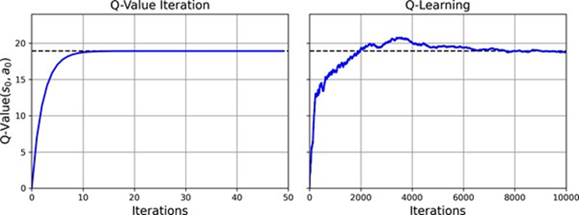
\includegraphics[width=\textwidth,height=0.6\textheight,keepaspectratio]{../machineLearningWeb/Figures/CH18/Hình_18-9.png}
            \vspace{0.2cm}
            \textit{Hình 18-9: Quá trình leo dốc tối ưu hàm mục tiêu J(theta)}
        \end{column}
    \end{columns}
\end{frame}

% 35
\begin{frame}{5.4 Vấn đề Phương sai (High Variance) của REINFORCE}
    \begin{itemize}
        \item Vấn đề lớn nhất của REINFORCE là phương sai cực kỳ lớn.
        \item Cùng một chuỗi hành động ngẫu nhiên, có khi gặp may mắn được 100 điểm, có khi gặp xui xẻo được -10 điểm. Việc phạt/thưởng mù quáng khiến quá trình huấn luyện mất ổn định.
        \item Giải pháp: Sử dụng \textbf{Đường Cơ sở (Baseline)}. Thay vì nhìn vào $G_t$, ta nhìn vào $(G_t - b)$. Tức là "Hành động này có mang lại lợi nhuận cao hơn MỨC TRUNG BÌNH không?".
    \end{itemize}
\end{frame}


%==================================================================
\section{6. Actor-Critic và Các Kiến trúc Hiện đại}
%==================================================================

% 36
\begin{frame}{6.1 Khái niệm Actor-Critic (Diễn viên \& Nhà Phê Bình)}
    \begin{columns}
        \begin{column}{0.4\textwidth}
            \begin{itemize}
                \item Kết hợp đỉnh cao của 2 thế giới:
                \item \textbf{Actor (PG):} Mạng chính sách quyết định hành động.
                \item \textbf{Critic (Q-Learning):} Mạng giá trị đánh giá hành động đó được mấy điểm.
                \item Actor đưa ra quyết định $\rightarrow$ Critic chấm điểm $\rightarrow$ Actor dùng điểm đó làm Baseline để tự sửa đổi.
            \end{itemize}
        \end{column}
        \begin{column}{0.6\textwidth}
            \centering
            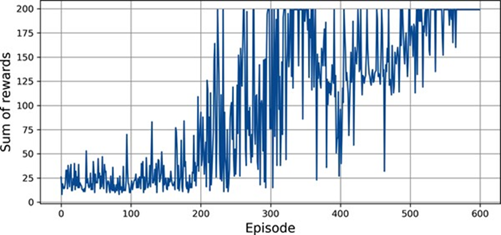
\includegraphics[width=\textwidth,height=0.65\textheight,keepaspectratio]{../machineLearningWeb/Figures/CH18/Hình_18-10.png}
            \vspace{0.2cm}
            \textit{Hình 18-10: Cấu trúc thuật toán Actor-Critic vòng lặp khép kín}
        \end{column}
    \end{columns}
\end{frame}

% 37
\begin{frame}{6.2 Ưu điểm của Actor-Critic}
    \begin{itemize}
        \item Giải quyết bài toán phương sai cao của REINFORCE (nhờ Critic).
        \item Xử lý được cả không gian trạng thái liên tục và rời rạc.
        \item Hội tụ cực kỳ nhanh so với DQN thuần túy.
        \item Hầu hết các thành tựu AI lớn nhất thập kỷ qua (AlphaStar chơi Starcraft 2, OpenAI Five chơi Dota 2) đều dùng kiến trúc bắt nguồn từ Actor-Critic.
    \end{itemize}
\end{frame}

% 38
\begin{frame}{6.3 Thuật toán A3C (Asynchronous Advantage Actor-Critic)}
    \begin{itemize}
        \item (DeepMind - 2016): Thay vì chỉ 1 Agent chơi game, ta thả 16, 32, hay 64 Agent con (Workers) chơi game ĐỒNG THỜI trên các luồng CPU khác nhau.
        \item Mỗi Agent tự chơi, tự tính Gradient, rồi gửi về Mạng Tổng (Global Network).
        \item Mạng Tổng chia sẻ lại kinh nghiệm cho các Agent con.
        \item Không cần Replay Buffer! Sự đa dạng từ các Agent con đã đủ để phá vỡ tính tương quan thời gian.
    \end{itemize}
\end{frame}

% 39
\begin{frame}{6.4 Thuật toán PPO (Proximal Policy Optimization)}
    \begin{itemize}
        \item PPO (OpenAI - 2017) hiện là thuật toán mặc định vàng (Gold Standard) cho Hầu hết bài toán Học Tăng Cường.
        \item Khắc phục nhược điểm "bước quá dài" của PG (nhảy quá tay mất luôn cực đại).
        \item Cắt xén (Clipping) vùng thay đổi, ép trọng số mạng không được thay đổi quá 20\% mỗi lần cập nhật.
        \item Đây chính là thuật toán dùng trong RLHF để tạo ra ChatGPT!
    \end{itemize}
\end{frame}


%==================================================================
\section{7. Tổng kết}
%==================================================================

% 40
\begin{frame}{Tổng Kết Chương 18}
    \begin{itemize}
        \item Học Tăng Cường mang lại trí thông minh thực sự linh hoạt cho Robot và Phần mềm, khác hẳn Học có giám sát.
        \item \textbf{Value-based (Q-Learning, DQN):} Học cách chấm điểm các trạng thái, phù hợp cho bài toán rời rạc. Cần dùng Replay Buffer \& Target Network.
        \item \textbf{Policy-based (REINFORCE, PPO):} Tối ưu hóa trực tiếp xác suất hành động, phù hợp cho điều khiển liên tục.
        \item Sự hội tụ của 2 trường phái tạo ra \textbf{Actor-Critic}, xương sống của AI tiên tiến nhất ngày nay.
    \end{itemize}
\end{frame}

% 41
\begin{frame}
    \centering
    \Huge \textbf{HỎI \& ĐÁP}
\end{frame}

\end{document}
